%%%%%%%%%%%%%%%%%%%%%%%%%%%%%%%%%%%%%%%%%%%%%%%%%%%%%%%%%%%%%%%%%%%%%%
% Overleaf (WriteLaTeX) Example: Molecular Chemistry Presentation
%
% Source: http://www.overleaf.com
%
% In these slides we show how Overleaf can be used with standard 
% chemistry packages to easily create professional presentations.
% 
% Feel free to distribute this example, but please keep the referral
% to overleaf.com
% 
%%%%%%%%%%%%%%%%%%%%%%%%%%%%%%%%%%%%%%%%%%%%%%%%%%%%%%%%%%%%%%%%%%%%%%
% How to use Overleaf: 
%
% You edit the source code here on the left, and the preview on the
% right shows you the result within a few seconds.
%
% Bookmark this page and share the URL with your co-authors. They can
% edit at the same time!
%
% You can upload figures, bibliographies, custom classes and
% styles using the files menu.
%
% If you're new to LaTeX, the wikibook is a great place to start:
% http://en.wikibooks.org/wiki/LaTeX
%
%%%%%%%%%%%%%%%%%%%%%%%%%%%%%%%%%%%%%%%%%%%%%%%%%%%%%%%%%%%%%%%%%%%%%%

\documentclass{beamer}

% For more themes, color themes and font themes, see:
% http://deic.uab.es/~iblanes/beamer_gallery/index_by_theme.html
%
\mode<presentation>
{
  \usetheme{Madrid}       % or try default, Darmstadt, Warsaw, ...
  \usecolortheme{default} % or try albatross, beaver, crane, ...
  \usefonttheme{serif}    % or try default, structurebold, ...
  \setbeamertemplate{navigation symbols}{}
  \setbeamertemplate{caption}[numbered]
} 

\usepackage[english]{babel}
\usepackage[utf8x]{inputenc}
\usepackage{chemfig}
\usepackage[version=3]{mhchem}
%allows for strikeout:
\usepackage[normalem]{ulem}
% On Overleaf, these lines give you sharper preview images.
% You might want to `comment them out before you export, though.
\usepackage{pgfpages}
\usepackage{hyperref}
\hypersetup{
    colorlinks=false,
    linkcolor=blue,
    filecolor=magenta,      
    urlcolor=cyan,
}
\pgfpagesuselayout{resize to}[%
  physical paper width=8in, physical paper height=6in]

% Here's where the presentation starts, with the info for the title slide
\title[Unraveling]{Unraveling as Endogenous Market Thinness}
\author{Tyler Hoppenfeld}
\institute{UC Davis}
\date{\today}

\newtheorem{thm}{Theorm}
\newtheorem{prop}{Proposition}

\newtheorem{deff}{Definition}
\usepackage{graphicx}
\graphicspath{ {../} }
\begin{document}

\begin{frame}
  \titlepage
\end{frame}

% These three lines create an automatically generated table of contents.
\begin{frame}{Outline}
  \tableofcontents
\end{frame}

\section{Introduction}
\subsection{Dysfunctional Markets}
\begin{frame}{Law Clerkships}

\begin{itemize}
  \item The very best law school graduates want high-prestige clerkships
  \item The very best judges would like to hire the very best graduates as clerks
  \item All of these positions are filled after summer of 1st year. (Law school is 3 years)
\end{itemize}

\end{frame}

\subsection{Functional Markets}
\begin{frame}{Medical Residencies}

\begin{itemize}
\item The very best medical school graduates want high-prestige residencies
\item The very best residencies would like to hire the very best graduates as residents
\item This market clears smoothly with an orderly centralized deferred acceptance process
\end{itemize}
\end{frame}


\subsection{State of Literature}

\begin{frame}{Past Research}
\begin{itemize}
\item Past modeling of unraveling uses:
\begin{itemize}
    \item Risk aversion
    \item  Cost of using match process (ie, frictions)
\end{itemize}
\item Past empirical work appeals to stability of matching
\begin{itemize}
    \item It is a usually true various medical matching markets that if the process gives a  \hyperlink{definestable}{stable} \hypertarget{r_definestable}{allocation}, it works
    \item That said, some markets with stable allocations have still unraveled (eg, GI fellowships)
\end{itemize}
\end{itemize}
\end{frame}

\begin{frame}{Past Research}
\begin{itemize}
\item Fails to capture ``endogenous market thinness"
\item Do not explain why some stable clearinghouses fail
\end{itemize}


\end{frame}


\section{Model}
\subsection{Model Goals}

\begin{frame}{Model Goals}
\begin{itemize}
    \item Friction-less access to stable matching
    \item Stability at unraveled state
    \item Stable matching pareto preferred to unraveled state
\end{itemize}
\end{frame}


\begin{frame}{Outline}
	\tableofcontents
\end{frame}

\subsection{Model Design}

\begin{frame}{Model Outline}
    \begin{itemize}
        \item <1-> Two-Period Model 
        \item <2-> Two types of agents
        \begin{itemize}
            \item Buyers (eg. employers)
            \item Sellers (eg. employees)
        \end{itemize}
        \item <3-> First period random matching, opportunity to contract and exit market
        \item <4-> Second period DA with fixed contracts
    \end{itemize}
\end{frame}
\begin{frame}{Agents}
\begin{itemize}
    \item Sellers mass 1, indexed $i \in (0,1]$
    \item  Buyers mass 1, ex ante homogeneous, indexed $j \in (0,1]$
\end{itemize}
\end{frame}

\begin{frame}{Valuations}
\begin{itemize}
    \item  When buyer and seller contract, a surplus of $i + \alpha \epsilon_{ij}$ is generated
    \item For each Buyer/Seller pair $\epsilon_{ij}$ is randomly drawn from Uniform $[0,1]$
\end{itemize}
\end{frame}


\begin{frame}{Mechanics}
    \begin{itemize}
    \item <1-> In period 1, buyers and sellers are matched randomly. Buyer has opportunity to make TIOLI offer.  If they do not contract, they both move on to the next period.
    \item <2-> In period 2, remaining buyers and sellers engage in a deferred acceptance market. In this DA market, buyer receives a fixed share $\eta$ of the surplus from trade

\end{itemize}
\end{frame}

\subsection{Model Solution}

\begin{frame}{First Understand Period 2}
\begin{lemma} \label{lemma:e_1}
	%For any buyer and seller ${s_i, b_j}$ matched in period 2 such that $i \neq 0$ , $\epsilon_{ij} = 1$
	For any buyer and seller $\{s_i, b_j\}$ matched in period 2: 
	 $$\epsilon_{ij} = 1$$
\end{lemma}

\begin{deff}
	$\omega(i) $ is the probability that seller $s_i$ has chosen to proceed to period 2
	
\end{deff}
\end{frame}


\begin{frame}{Period 2 Outcomes}
\begin{lemma}
	%	Each seller $s_i, i>0$ who proceeds to period 2 expects a payoff of $\eta (i+\alpha)$
	Each seller $s_i$ who proceeds to period 2 expects a payoff of 
	\begin{equation}
	\eta (i+\alpha)
	\end{equation}
	
\end{lemma}

\begin{lemma}
	%if any measure of buyers and sellers proceed to period two
	Each buyer expects a payoff of 
	\begin{equation} \label{eq:E_buyer}
	\eta  \left[ \frac{\int_0^1 \hat{i} \omega(\hat{i}) d\hat{i}}{\int_0^1  \omega(\hat{i}) d\hat{i} } + \alpha \right]
	\end{equation}
\end{lemma}

\end{frame}
\begin{frame}{Period 1 Outcomes}
	\begin{lemma}
		%	Each seller $s_i, i>0$ who proceeds to period 2 expects a payoff of $\eta (i+\alpha)$
		Agents $i$ and $j$ matched in period 1 will contract early if:
		\begin{equation} \label{eq:ec_condition_raw}
		i+\alpha \epsilon_{ij} >(1-\eta)(i+\alpha ) + \eta  \left[ \frac{\int_0^1 \hat{i} \omega(\hat{i}) di}{\int_0^1  \omega(\hat{i}) d\hat{i}} + \alpha \right] 
		\end{equation}
	\end{lemma}



\end{frame}


\begin{frame}{Guess and Verify}
\begin{itemize}
\item First see that for each value of $i$, there is some value $\epsilon^* (i)$ such that inequality \ref{eq:ec_condition_raw} is satisfied iff $\epsilon_{ij} > \epsilon^* (i)$ 
\begin{equation} \label{eq:e_star_unsolved}
\epsilon^*(i) = (1-\eta) + \frac{   \eta \left[ \frac{\int_0^1 \hat{i} \omega(\hat{i}) di}{\int_0^1  \omega(\hat{i}) d\hat{i}} + \alpha -i \right] }{\alpha} 
\end{equation}

\item Guess:
 \begin{equation} \label{eq:e_star_guess}
\epsilon^*(i) = a-\frac{\eta }{\alpha}i
\end{equation} 


for  $a \in [0,1+\frac{\eta }{\alpha}]$
\end{itemize}
\end{frame}

\begin{frame}{Elaborate on $\omega(\cdot)$}
	As we have specified that $\epsilon_{ij} ~ U[0,1]$, we also can note that 
	
	\begin{equation} \label{eq:omega_epsilon}
	\omega(i) =
	\begin{cases}
	0 |  \epsilon^* (i) < 0 \\
	\epsilon^* (i) | \epsilon^* (i) \in [0,1] \\
	1 |  \epsilon^* (i) > 1
	\end{cases}
	\end{equation}
	
	
	
\end{frame}

\begin{frame}{The Part Where I Skip The Algebra}
Combining equations \ref{eq:e_star_unsolved}, \ref{eq:e_star_guess} and \ref{eq:omega_epsilon}, I find:

\begin{equation} \label{eq:big_reveal}
\epsilon^*(i) = 1 - \frac{\sqrt{3}}{3} - \frac{\eta}{\alpha} i
\end{equation}

(* This is almost but not quite true)
\end{frame}

\begin{frame}{Outline}
	\tableofcontents
\end{frame}

\section{Comparative Statics}
\subsection{Sufficient Statistic}
\begin{frame}{ $\epsilon^*(i)$ is a sufficient statistic}
	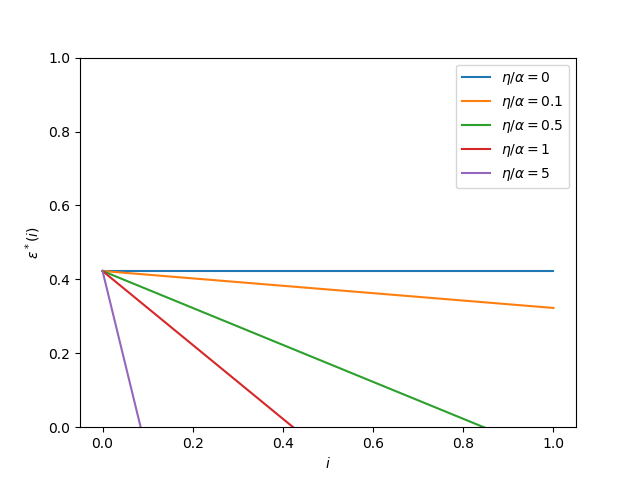
\includegraphics[width=0.9\textwidth]{epsilon_graph}
	
\end{frame}

\subsection{Welfare}
\begin{frame}{Welfare}
	\begin{itemize}
		\item TIOLI structure means sellers are unaffected by unraveling
		\item Buyers are worse off because of unraveling
		\begin{itemize}
			\item Haven't quantified this yet, but since Sellers see no welfare change and the realized values of $\epsilon_{ij}$ are lower, this is clear
		\end{itemize}
	\end{itemize}
\end{frame}

\subsection{Endogenous Thinness}
\begin{frame}{Endogenous Component}
The next step here is to identify how much early contracting is caused by the endogenous of:
$$	\eta  \left[ \frac{\int_0^1 \hat{i} \omega(\hat{i}) d\hat{i}}{\int_0^1  \omega(\hat{i}) d\hat{i} } + \alpha \right]$$
\end{frame}




\begin{frame}{Defining Stability}

A \hypertarget{definestable}{stable} matching is a matching between the two sides of the market that is
\begin{enumerate}
    \item feasible 
    \item individually rational
        \begin{itemize}
            \item no agent would prefer to be unmatched 
        \end{itemize}
    \item free of blocking pairs
    \begin{itemize}
        \item no two agents would prefer to be matched to each other instead of their current assignments
    \end{itemize}
\end{enumerate}

\hyperlink{r_definestable}{Return}
\end{frame}


\end{document}